\documentclass{beamer}
\usepackage{beamerthemeshadow}
\beamertemplatetransparentcovereddynamic
\usepackage{graphicx}
\usepackage{amsmath}
\usepackage{algorithm}
\usepackage{algorithmic}

%PSO Stuff
\DeclareMathOperator{\URand}{U}
\providecommand{\ppos}{\ensuremath{\Vec{x}}}
\providecommand{\pvel}{\ensuremath{\Vec{v}}}
\providecommand{\nbest}{\ensuremath{\Vec{b}_n}}
\providecommand{\pbest}{\ensuremath{\Vec{b}_p}}
\providecommand{\constriction}{\ensuremath{\chi}}
\providecommand{\coeff}{\ensuremath{\phi}}

%SpecExPSO Stuff
\providecommand{\noeval}[1]{\ensuremath{#1^{-e}}}
\providecommand{\nonbest}[1]{\ensuremath{#1^{-n}}}
\providecommand{\p}{\ensuremath{p}}
\providecommand{\pset}{\ensuremath{\mathbf{p}}}
\providecommand{\s}{\ensuremath{s}}
\providecommand{\sset}{\ensuremath{\mathbf{s}}}
\providecommand{\nsset}{\ensuremath{\mathbf{ns}}}
\providecommand{\n}{\ensuremath{n}}
\providecommand{\nset}{\ensuremath{\mathbf{n}}}
\providecommand{\nnset}{\ensuremath{\mathbf{nn}}}

\title{A Speculative Approach to Parallelization in Particle Swarm Optimization}
\author{Matthew Gardner}
\date{\today}

\begin{document}
\begin{frame}
  \titlepage
\end{frame}

\section{Optimization}
\begin{frame}
  \frametitle{Optimization}
  \includegraphics[width=\textwidth]{cosine}
\end{frame}

\section{Particle Swarm Optimization}
\subsection{Basic Idea}
\begin{frame}
  \frametitle{Particle Swarm Optimization}
  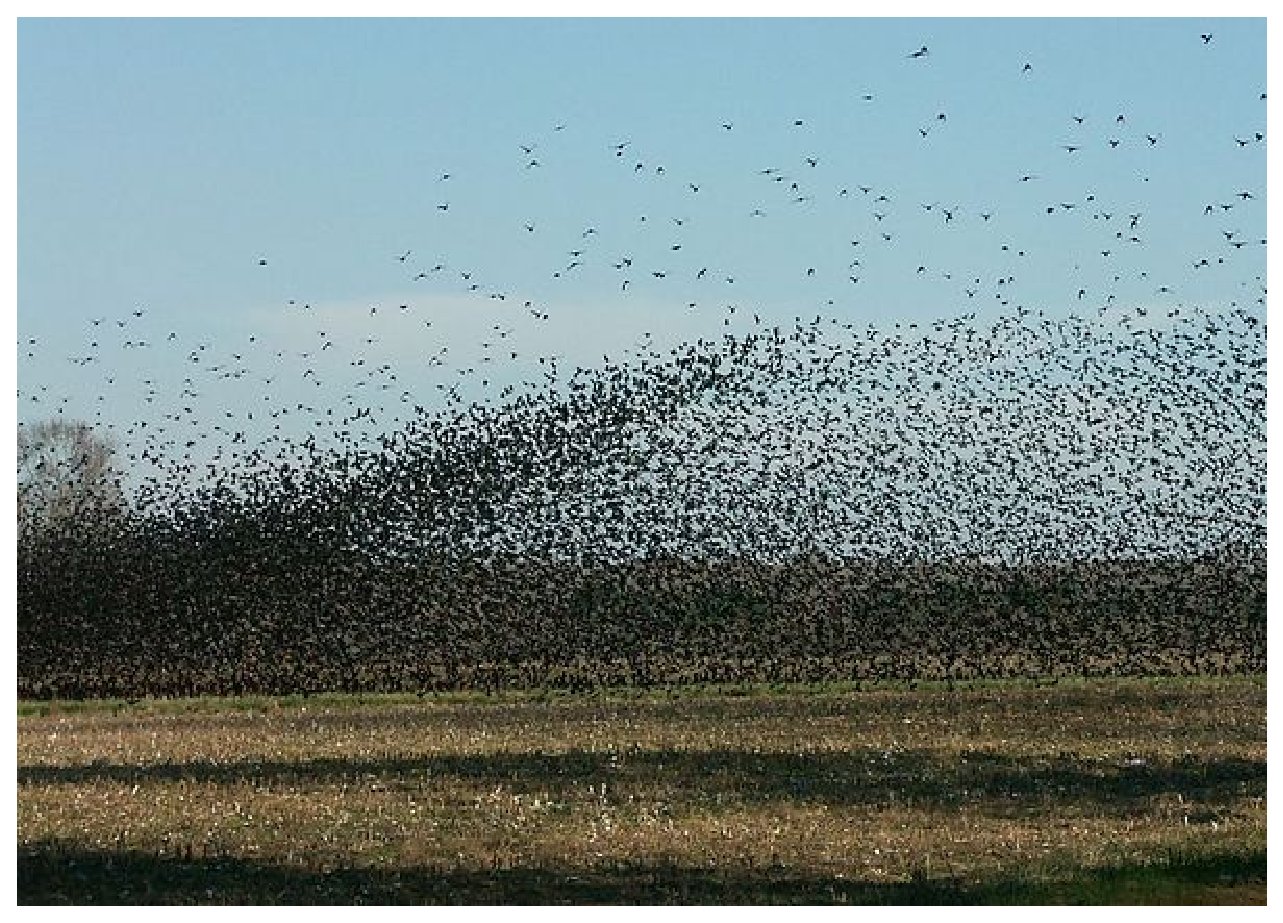
\includegraphics[width=\textwidth]{birds}
\end{frame}

\subsection{The Math}
\begin{frame}
  \frametitle{PSO Equations}
  \begin{align*}
	  \pvel_{t+1} &=
		  \constriction \left[ \pvel_t +
			  \coeff_1\URand()\otimes(\pbest - \ppos_t) +
			  \coeff_2\URand()\otimes(\nbest - \ppos_t)
		  \right] \\
	  \ppos_{t+1} &= \ppos_t + \pvel_{t+1}
  \end{align*}
\end{frame}

\subsection{Who's My Neighbor?}
\begin{frame}
  \frametitle{Who's My Neighbor?}
  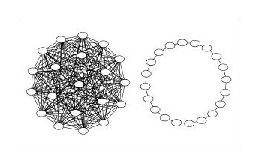
\includegraphics[width=\textwidth]{gbest_and_lbest}
\end{frame}

\subsection{No Free Lunch}
\begin{frame}
  \frametitle{No Free Lunch!}
  
\includegraphics[width=.6\textwidth]{no-free-lunch}
\end{frame}

\section{Speculative Evaluation}

\subsection{Speculative Execution}
\begin{frame}
  \frametitle{Speculative Execution}
  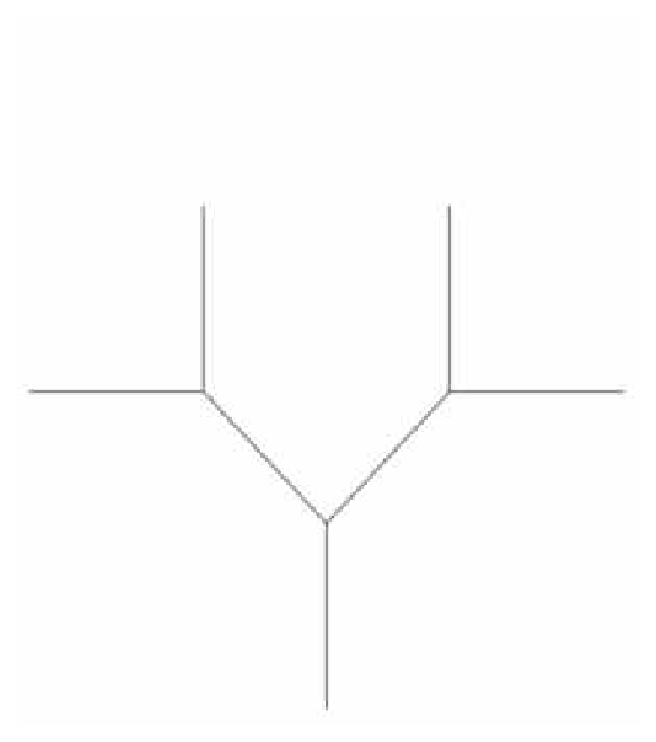
\includegraphics[width=\textwidth]{branching}
\end{frame}

\subsection{Speculative Evaluation in PSO}
\begin{frame}
  \frametitle{Speculative Evaluation in PSO}
  \begin{align*}
	  \pvel_{t+1} &=
		  \constriction \left[ \pvel_t +
			  \coeff_1\URand()\otimes(\pbest - \ppos_t) +
			  \coeff_2\URand()\otimes(\nbest - \ppos_t)
		  \right]
  \end{align*}
  \pause
  \begin{center}
	\begin{tabular}{cc}
	  $\pbest$ updated&Source of $\nbest$ update\\
	  \hline
	  \hline
	  No update&No update\\
	  \hline
	  No update&Neighbor 1\\
	  \hline
	  No update&Neighbor 2\\
	  \hline
	  Updated&No update\\
	  \hline
	  Updated&Neighbor 1\\
	  \hline
	  Updated&Neighbor 2\\
	  \hline
	  Updated&The particle itself\\
	  \hline
	\end{tabular}
  \end{center}
\end{frame}

\begin{frame}
  \begin{center}
\begin{algorithm}[H]
  \caption{Speculative Evaluation in a Centralized PSO}
  \label{alg:centralized}
  \begin{algorithmic}[1]
	\STATE Move all $\p_{t-1}$ to $\noeval{\p}_t$
	\STATE For each $\noeval{\p}_t$, get its neighbors $\noeval{\nset}_t$ and
	  generate $\noeval{\sset}_{t+1}$
	\STATE Evaluate all $\noeval{\p}_t$ and $\noeval{\sset}_{t+1}$ in parallel
	\STATE Update personal best for each $\noeval{\p}_t$ and
	  $\noeval{\s}_{t+1}$, creating $\nonbest{\p}_t$ and $\nonbest{\s}_{t+1}$
	\STATE Update neighborhood best for each $\nonbest{\p}_t$, creating
	  $\pset_t$
	\FORALL{$\p_t$}
	\STATE Pick $\nonbest{\s}_{t+1}$ from $\nonbest{\sset}_{t+1}$ that matches
	the branch taken by $\p_t$ \\ (Or, pick $\nonbest{\s}_{t+1}$ from
	$\nonbest{\sset}_{t+1}$ that has the highest value)
	\STATE Pass along personal and neighborhood best values obtained by $\p_t$,
	  making $\nonbest{\p}_{t+1}$
	\ENDFOR
	\STATE Update neighborhood best for each $\nonbest{\p}_{t+1}$, creating
	  $\pset_{t+1}$
	\STATE Repeat
  \end{algorithmic}
\end{algorithm}
  \end{center}
\end{frame}

\subsection{Results}
\begin{frame}
  \begin{center}
	\frametitle{Results---Sphere}
	\[f(\Vec{x}) = \sum_{i=1}^D x_i^2\]
	\includegraphics[width=.6\textwidth]{sphere1}
  \end{center}
\end{frame}
\begin{frame}
  \begin{center}
	\frametitle{Results---Griewank (240 Processors)}
	\[f(\Vec{x}) = \frac{1}{4000} \sum_{i=1}^D x_i^2 - \Pi_{i=1}^D
	\cos\left(\frac{x_i}{\sqrt{i}}\right) + 1\]
	\includegraphics[width=.6\textwidth]{griewank1}
  \end{center}
\end{frame}
\begin{frame}
  \begin{center}
	\frametitle{Results---Griewank (800 Processors)}
	\[f(\Vec{x}) = \frac{1}{4000} \sum_{i=1}^D x_i^2 - \Pi_{i=1}^D
	\cos\left(\frac{x_i}{\sqrt{i}}\right) + 1\]
	\includegraphics[width=.6\textwidth]{griewank2}
  \end{center}
\end{frame}
\begin{frame}
  \begin{center}
	\frametitle{Results---Rastrigin}
	\[f(\Vec{x}) = \sum_{i=1}^D \left(x_i^2 - 10\cos\left(2\pi x_i\right) +
	10\right)\]
	\includegraphics[width=.6\textwidth]{rastrigin}
  \end{center}
\end{frame}

\begin{frame}
  \frametitle{Questions?}
  \begin{center}
	\Huge \textrm{The End}
  \end{center}
\end{frame}

\end{document}
